\documentclass[12pt,a4paper]{article}

% Packages
\usepackage[utf8]{inputenc}
\usepackage[french]{babel}
\usepackage[T1]{fontenc}
\usepackage{geometry}
\usepackage{graphicx}
\usepackage{hyperref}
\usepackage{listings}
\usepackage{xcolor}
\usepackage{float}
\usepackage{booktabs}
\usepackage{caption}
\usepackage{subcaption}
\usepackage{fancyhdr}
\usepackage{titlesec}
\usepackage{amsmath}
\usepackage{amssymb}

% Geometry
\geometry{left=2.5cm, right=2.5cm, top=3cm, bottom=3cm}

% Hyperref setup
\hypersetup{
    colorlinks=true,
    linkcolor=blue,
    filecolor=magenta,      
    urlcolor=cyan,
    citecolor=green,
}

% Code listing setup
\lstdefinestyle{sqlstyle}{
    language=SQL,
    basicstyle=\ttfamily\footnotesize,
    keywordstyle=\color{blue}\bfseries,
    commentstyle=\color{green!60!black}\itshape,
    stringstyle=\color{red},
    numbers=left,
    numberstyle=\tiny\color{gray},
    stepnumber=1,
    numbersep=8pt,
    backgroundcolor=\color{gray!10},
    showspaces=false,
    showstringspaces=false,
    showtabs=false,
    frame=single,
    tabsize=2,
    captionpos=b,
    breaklines=true,
    breakatwhitespace=false,
}

\lstdefinestyle{pythonstyle}{
    language=Python,
    basicstyle=\ttfamily\footnotesize,
    keywordstyle=\color{blue}\bfseries,
    commentstyle=\color{green!60!black}\itshape,
    stringstyle=\color{orange},
    numbers=left,
    numberstyle=\tiny\color{gray},
    stepnumber=1,
    numbersep=8pt,
    backgroundcolor=\color{gray!10},
    showspaces=false,
    showstringspaces=false,
    showtabs=false,
    frame=single,
    tabsize=4,
    captionpos=b,
    breaklines=true,
    breakatwhitespace=false,
}

% Header and footer
\pagestyle{fancy}
\fancyhf{}
\fancyhead[L]{TP1 - Gestion de Bases de Données}
\fancyhead[R]{M1 DENG}
\fancyfoot[C]{\thepage}

% Title formatting
\titleformat{\section}{\Large\bfseries}{\thesection.}{1em}{}
\titleformat{\subsection}{\large\bfseries}{\thesubsection.}{1em}{}

% Document
\begin{document}

% Page de garde
\begin{titlepage}
    \centering
    \vspace*{2cm}
    
    {\Huge\bfseries Conception et Optimisation d'une Base de Données\\de Gestion de la Recherche\par}
    
    \vspace{1.5cm}
    
    {\Large TP1 - Gestion de Bases de Données et Data Warehouse\par}
    
    \vspace{2cm}
    
    {\large Master 1 Data Engineering (M1 DENG)\par}
    
    \vspace{1cm}
    
    {\large Université de Corse\par}
    
    \vspace{3cm}
    
    {\large Réalisé par :\par}
    {\Large 
    Nom Prénom 1\\
    Nom Prénom 2\\
    Nom Prénom 3\par}
    
    \vfill
    
    {\large Date de rendu : 12 novembre 2025\par}
    
\end{titlepage}

% Table des matières
\tableofcontents
\newpage

% Introduction
\section{Introduction}

\subsection{Contexte du projet}
Ce projet s'inscrit dans le cadre du TP1 du module de Gestion de Bases de Données et Data Warehouse. L'objectif est de concevoir et implémenter une base de données relationnelle pour la gestion des données de recherche d'une université.

\subsection{Objectifs}
Les objectifs principaux, comme énoncés dans le sujet, sont :
\begin{itemize}
    \item Concevoir un schéma relationnel cohérent pour gérer les institutions, laboratoires, projets, chercheurs, contrats, publications et jeux de données
    \item Peupler la base avec des données fictives réalistes
    \item Implémenter une gestion sécurisée des accès via des rôles et des vues
    \item Optimiser les requêtes complexes
    \item Mettre en œuvre des triggers et procédures stockées
\end{itemize}

Ces objectifs seront développés dans les différentes parties de ce rapport.

\subsection{Organisation du rapport}
Ce rapport présente successivement :
\begin{itemize}
    \item La conception de la base de données (Partie 1) qui s'appuie sur l'utilisation d'outils d'IA générative.
    \item Le peuplement de la base (Partie 2)
    \item La gestion des utilisateurs et des vues (Partie 3)
    \item L'optimisation des requêtes (Partie 4)
    \item Les triggers et procédures stockées (Partie 5)
\end{itemize}

\newpage

% Partie 1
\section{Partie 1 - Conception de la Base de Données}

\subsection{Méthodologie et utilisation de l'IA générative}

\subsubsection{Outils utilisés}
La phase de conception a été assistée par l'agent de code Claude Sonnet 4.5 par le biais de l'extension Visual Studio Code "GitHub Copilot Chat".

Cet outil d'IA générative a principalement permis, à partir d'instructions et du contexte de l'environnement de développement, de proposer des suggestions de code, des structures de données, et d'aider à la modélisation conceptuelle, le tout par le biais de création de fichiers de façon automatique.

\subsubsection{Démarche adoptée}
\begin{enumerate}
    \item Analyse du cahier des charges
    \item Identification des entités et relations
    \item Validation et raffinement avec l'IA
    \item Analyse critique des propositions et corrections
\end{enumerate}

\subsubsection{Résultats}
L'IA a permis de générer une première version du schéma relationnel, incluant les tables, attributs, types de données et contraintes d'intégrité.

Après lui avoir donné le contexte de l'exercice et les exigences (par un simple copier-coller du cahier des charges), nous avons obtenu :
\begin{itemize}
    \item Un schéma relationnel complet
    \item Des descriptions détaillées des tables
    \item Des suggestions de contraintes d'intégrité
    \item Les requêtes SQL de création
    \item Un fichier .dbml pour visualiser le MCD
    \item Des règles métier et triggers de validation (que nous avons supprimés par la suite car non demandés, et non conformes au sujet du TP)
\end{itemize}

\subsubsection{Analyse critique}
L'utilisation de l'IA générative nous a été extrèmement utile pour obtenir une base solide, cohérente dans un temps très réduit. Les suggestions étaient globalement pertinentes et conformes au cahier des charges.

Nous avons rencontré cependant une limitation qui ne nous a pas réellement pénalisés : l'IA a pris volontairement la décision de simplifier la relation entre deux entités (Chercheur et Projet) en optant pour une relation 1-N au lieu de N-N (un chercheur ne pouvait être que dans un seul projet.. Or ce n'est pas réaliste et assez contraignant), ce qui n'était pas conforme au sujet. Nous avons corrigé cela en y ajoutant une table d'association.

\subsection{Interprétation du cahier des charges}

\subsubsection{Entités principales identifiées}
\begin{itemize}
    \item Institution
    \item Laboratoire
    \item Projet
    \item Chercheur
    \item Contrat
    \item Publication
    \item Jeu de données
\end{itemize}

\subsubsection{Relations entre entités}
\begin{itemize}
    \item \textbf{Institution $\rightarrow$ Laboratoire} : Une institution héberge un ou plusieurs laboratoires (1-N). Chaque laboratoire appartient à une seule institution;
    
    \item \textbf{Laboratoire $\rightarrow$ Projet} : Un laboratoire pilote un ou plusieurs projets (1-N). Chaque projet a un laboratoire pilote unique;
    
    \item \textbf{Laboratoire $\rightarrow$ Chercheur} : Un laboratoire regroupe plusieurs chercheurs (1-N). Chaque chercheur est rattaché à un laboratoire;
    
    \item \textbf{Projet $\leftrightarrow$ Chercheur} : Relation N-N modélisée par la table d'association \texttt{projet\_chercheur}. Un projet peut impliquer plusieurs chercheurs, et un chercheur peut participer à plusieurs projets. Cette table permet de gérer le rôle, la période de participation et le pourcentage d'effort de chaque chercheur sur chaque projet;
    
    \item \textbf{Projet $\rightarrow$ Chercheur (responsable)} : Un projet a un chercheur responsable (1-1 optionnel). Un chercheur peut être responsable de plusieurs projets;
    
    \item \textbf{Projet $\rightarrow$ Contrat} : Un projet peut être financé par plusieurs contrats (1-N). Chaque contrat finance un seul projet;
    
    \item \textbf{Contrat $\rightarrow$ Jeu\_Donnees} : Un contrat peut générer plusieurs jeux de données (1-N). Chaque jeu de données est associé à un unique contrat;
    
    \item \textbf{Chercheur $\rightarrow$ Jeu\_Donnees} : Un chercheur peut produire plusieurs jeux de données (1-N). Chaque jeu de données a un auteur principal unique;
    
    \item \textbf{Publication $\leftrightarrow$ Chercheur} : Relation N-N modélisée par la table d'association \texttt{publication\_auteur}. Une publication peut avoir plusieurs auteurs, et un chercheur peut publier plusieurs articles. L'attribut \texttt{ordre\_auteur} permet de gérer l'ordre de signature.
\end{itemize}


\subsubsection{Hypothèses et choix de conception}
Selon nos connaissances sur le domaine de la recherche académique, nous avons fait les choix suivants :
\begin{itemize}
    \item Un chercheur peut participer à plusieurs projets simultanément;
    \item Un projet peut avoir plusieurs chercheurs responsables (co-responsables) mais pour simplifier, nous avons choisi un seul responsable principal;
    \item Les publications ne sont pas directement rattachées aux projets, mais aux chercheurs. Cela reflète mieux la réalité où les chercheurs publient indépendamment de leurs projets;
    \item Les jeux de données sont liés aux contrats car ils résultent souvent des financements obtenus;
    \item Les types énumérés (ENUM) ont été définis pour les attributs avec des valeurs limitées (type d'institution, type de contrat, statut DMP).
\end{itemize}

\subsubsection{Dictionnaire des attributs}

Le dictionnaire nous a permis de clarifier le rôle de chaque table et attribut, ainsi que les contraintes associées.

\paragraph{Types énumérés}

\textbf{type\_institution :}
\begin{itemize}
    \item \texttt{universite} : Université
    \item \texttt{organisme\_recherche} : Organisme de recherche
    \item \texttt{partenaire\_prive} : Partenaire privé
\end{itemize}

\textbf{type\_contrat :}
\begin{itemize}
    \item \texttt{ANR} : Agence Nationale de la Recherche
    \item \texttt{H2020} : Horizon 2020 (programme européen)
    \item \texttt{Region} : Financement régional
    \item \texttt{Europe} : Financement européen
    \item \texttt{Autre} : Autre type de financement
\end{itemize}

\textbf{statut\_dmp :}
\begin{itemize}
    \item \texttt{brouillon} : DMP en cours de rédaction
    \item \texttt{soumis} : DMP soumis pour validation
    \item \texttt{valide} : DMP validé
\end{itemize}

\paragraph{Table Institution}
Institution de rattachement (université, organisme de recherche ou partenaire privé).

\begin{table}[H]
\centering
\small
\begin{tabular}{@{}llp{6cm}@{}}
\toprule
\textbf{Attribut} & \textbf{Type} & \textbf{Description} \\ \midrule
id & bigint & Identifiant unique (PK, auto-increment) \\
nom & text & Nom de l'institution (NOT NULL) \\
type\_institution & type\_institution & Type d'institution (NOT NULL, enum) \\
adresse & text & Adresse postale de l'institution \\ \bottomrule
\end{tabular}
\caption{Attributs de la table Institution. Mise en forme LaTeX par une IA générative.}
\end{table}


\paragraph{Table Laboratoire}
Laboratoire de recherche rattaché à une institution.

\begin{table}[H]
\centering
\small
\begin{tabular}{@{}llp{6cm}@{}}
\toprule
\textbf{Attribut} & \textbf{Type} & \textbf{Description} \\ \midrule
id & bigint & Identifiant unique (PK, auto-increment) \\
nom & text & Nom du laboratoire (NOT NULL) \\
id\_institution & bigint & FK vers Institution (NOT NULL) \\ \bottomrule
\end{tabular}
\caption{Attributs de la table Laboratoire. Mise en forme LaTeX par une IA générative.}
\end{table}


\paragraph{Table Projet}
Projet de recherche structurant dirigé par un chercheur unique.

\begin{table}[H]
\centering
\small
\begin{tabular}{@{}llp{5cm}@{}}
\toprule
\textbf{Attribut} & \textbf{Type} & \textbf{Description} \\ \midrule
id & bigint & Identifiant unique (PK) \\
titre & text & Titre du projet (NOT NULL) \\
description & text & Description détaillée \\
discipline & text & Discipline scientifique (NOT NULL) \\
budget\_annuel\_eur & decimal(12,2) & Budget annuel $\geq$ 0 (NOT NULL) \\
date\_debut & date & Date de début (NOT NULL) \\
date\_fin & date & Date de fin $\geq$ date\_debut \\
id\_laboratoire\_pilote & bigint & FK vers Laboratoire (NOT NULL) \\
id\_chercheur\_responsable & bigint & FK vers Chercheur \\ \bottomrule
\end{tabular}
\caption{Attributs de la table Projet. Mise en forme LaTeX par une IA générative.}
\end{table}


\paragraph{Table Chercheur}
Chercheur affilié à un laboratoire.

\begin{table}[H]
\centering
\small
\begin{tabular}{@{}llp{6cm}@{}}
\toprule
\textbf{Attribut} & \textbf{Type} & \textbf{Description} \\ \midrule
id & bigint & Identifiant unique (PK) \\
prenom & text & Prénom (NOT NULL) \\
nom & text & Nom (NOT NULL) \\
email & text & Email professionnel (NOT NULL, UNIQUE) \\
orcid & varchar(19) & Identifiant ORCID (UNIQUE) \\
discipline & text & Discipline de recherche \\
id\_laboratoire & bigint & FK vers Laboratoire (NOT NULL) \\ \bottomrule
\end{tabular}
\caption{Attributs de la table Chercheur. Mise en forme LaTeX par une IA générative.}
\end{table}

\paragraph{Table Projet\_Chercheur}
Table associative N-N entre projets et chercheurs.

\begin{table}[H]
\centering
\small
\begin{tabular}{@{}llp{5.5cm}@{}}
\toprule
\textbf{Attribut} & \textbf{Type} & \textbf{Description} \\ \midrule
id & bigint & Identifiant unique (PK) \\
id\_projet & bigint & FK vers Projet (NOT NULL) \\
id\_chercheur & bigint & FK vers Chercheur (NOT NULL) \\
role & text & Rôle dans le projet \\
date\_debut & date & Date de début de participation \\
date\_fin & date & Date de fin de participation \\
charge\_pct & decimal(5,2) & Pourcentage d'effort (0-100) \\
is\_principal & boolean & Chercheur principal (défaut: false) \\ \bottomrule
\end{tabular}
\caption{Attributs de la table Projet\_Chercheur. Mise en forme LaTeX par une IA générative.}
\end{table}

\paragraph{Table Contrat}
Contrat de financement d'un projet.

\begin{table}[H]
\centering
\small
\begin{tabular}{@{}llp{5cm}@{}}
\toprule
\textbf{Attribut} & \textbf{Type} & \textbf{Description} \\ \midrule
id & bigint & Identifiant unique (PK) \\
type\_contrat & type\_contrat & Type de contrat (NOT NULL, enum) \\
financeur & text & Organisme financeur (NOT NULL) \\
intitule & text & Intitulé du contrat (NOT NULL) \\
montant\_eur & decimal(14,2) & Montant total $\geq$ 0 (NOT NULL) \\
duree\_mois & int & Durée en mois ($>$ 0) \\
date\_debut & date & Date de début (NOT NULL) \\
date\_fin & date & Date de fin (NOT NULL) \\
id\_projet & bigint & FK vers Projet (NOT NULL) \\
statut\_dmp & statut\_dmp & Statut DMP (NOT NULL) \\
date\_validation\_dmp & date & Date validation DMP \\
url\_document\_dmp & text & URL du document DMP \\ \bottomrule
\end{tabular}
\caption{Attributs de la table Contrat. Mise en forme LaTeX par une IA générative.}
\end{table}

\paragraph{Table Publication}
Publication scientifique (métadonnées uniquement).

\begin{table}[H]
\centering
\small
\begin{tabular}{@{}llp{6cm}@{}}
\toprule
\textbf{Attribut} & \textbf{Type} & \textbf{Description} \\ \midrule
id & bigint & Identifiant unique (PK) \\
titre & text & Titre de la publication (NOT NULL) \\
doi & text & Digital Object Identifier (UNIQUE) \\
date\_publication & date & Date de publication \\
nb\_pages & int & Nombre de pages ($>$ 0) \\
url\_externe & text & URL vers le document (ex: HAL) \\ \bottomrule
\end{tabular}
\caption{Attributs de la table Publication. Mise en forme LaTeX par une IA générative.}
\end{table}

\paragraph{Table Publication\_Auteur}
Table associative N-N entre publications et chercheurs.

\begin{table}[H]
\centering
\small
\begin{tabular}{@{}llp{6cm}@{}}
\toprule
\textbf{Attribut} & \textbf{Type} & \textbf{Description} \\ \midrule
id\_publication & bigint & FK vers Publication (NOT NULL) \\
id\_chercheur & bigint & FK vers Chercheur (NOT NULL) \\
ordre\_auteur & int & Ordre d'auteur ($>$ 0, NOT NULL) \\ \bottomrule
\end{tabular}
\caption{Attributs de la table Publication\_Auteur. Mise en forme LaTeX par une IA générative.}
\end{table}

\paragraph{Table Jeu\_Donnees}
Jeu de données produit dans le cadre d'un contrat.

\begin{table}[H]
\centering
\small
\begin{tabular}{@{}llp{5.5cm}@{}}
\toprule
\textbf{Attribut} & \textbf{Type} & \textbf{Description} \\ \midrule
id & bigint & Identifiant unique (PK) \\
id\_contrat & bigint & FK vers Contrat (NOT NULL) \\
description & text & Description du dataset (NOT NULL) \\
id\_auteur & bigint & FK vers Chercheur (NOT NULL) \\
conditions\_acces & text & Conditions d'accès \\
licence & text & Licence d'utilisation \\
date\_creation & date & Date de création du jeu de données \\
date\_depot & date & Date de dépôt officiel \\
url\_externe & text & URL vers l'entrepôt \\ \bottomrule
\end{tabular}
\caption{Attributs de la table Jeu\_Donnees. Mise en forme LaTeX par une IA générative.}
\end{table}


\subsection{Schéma relationnel}

\subsubsection{Vue d'ensemble}
Présentation du schéma relationnel complet (diagramme). Voir Figure \ref{fig:schema}.

\begin{figure}[H]
    \centering
    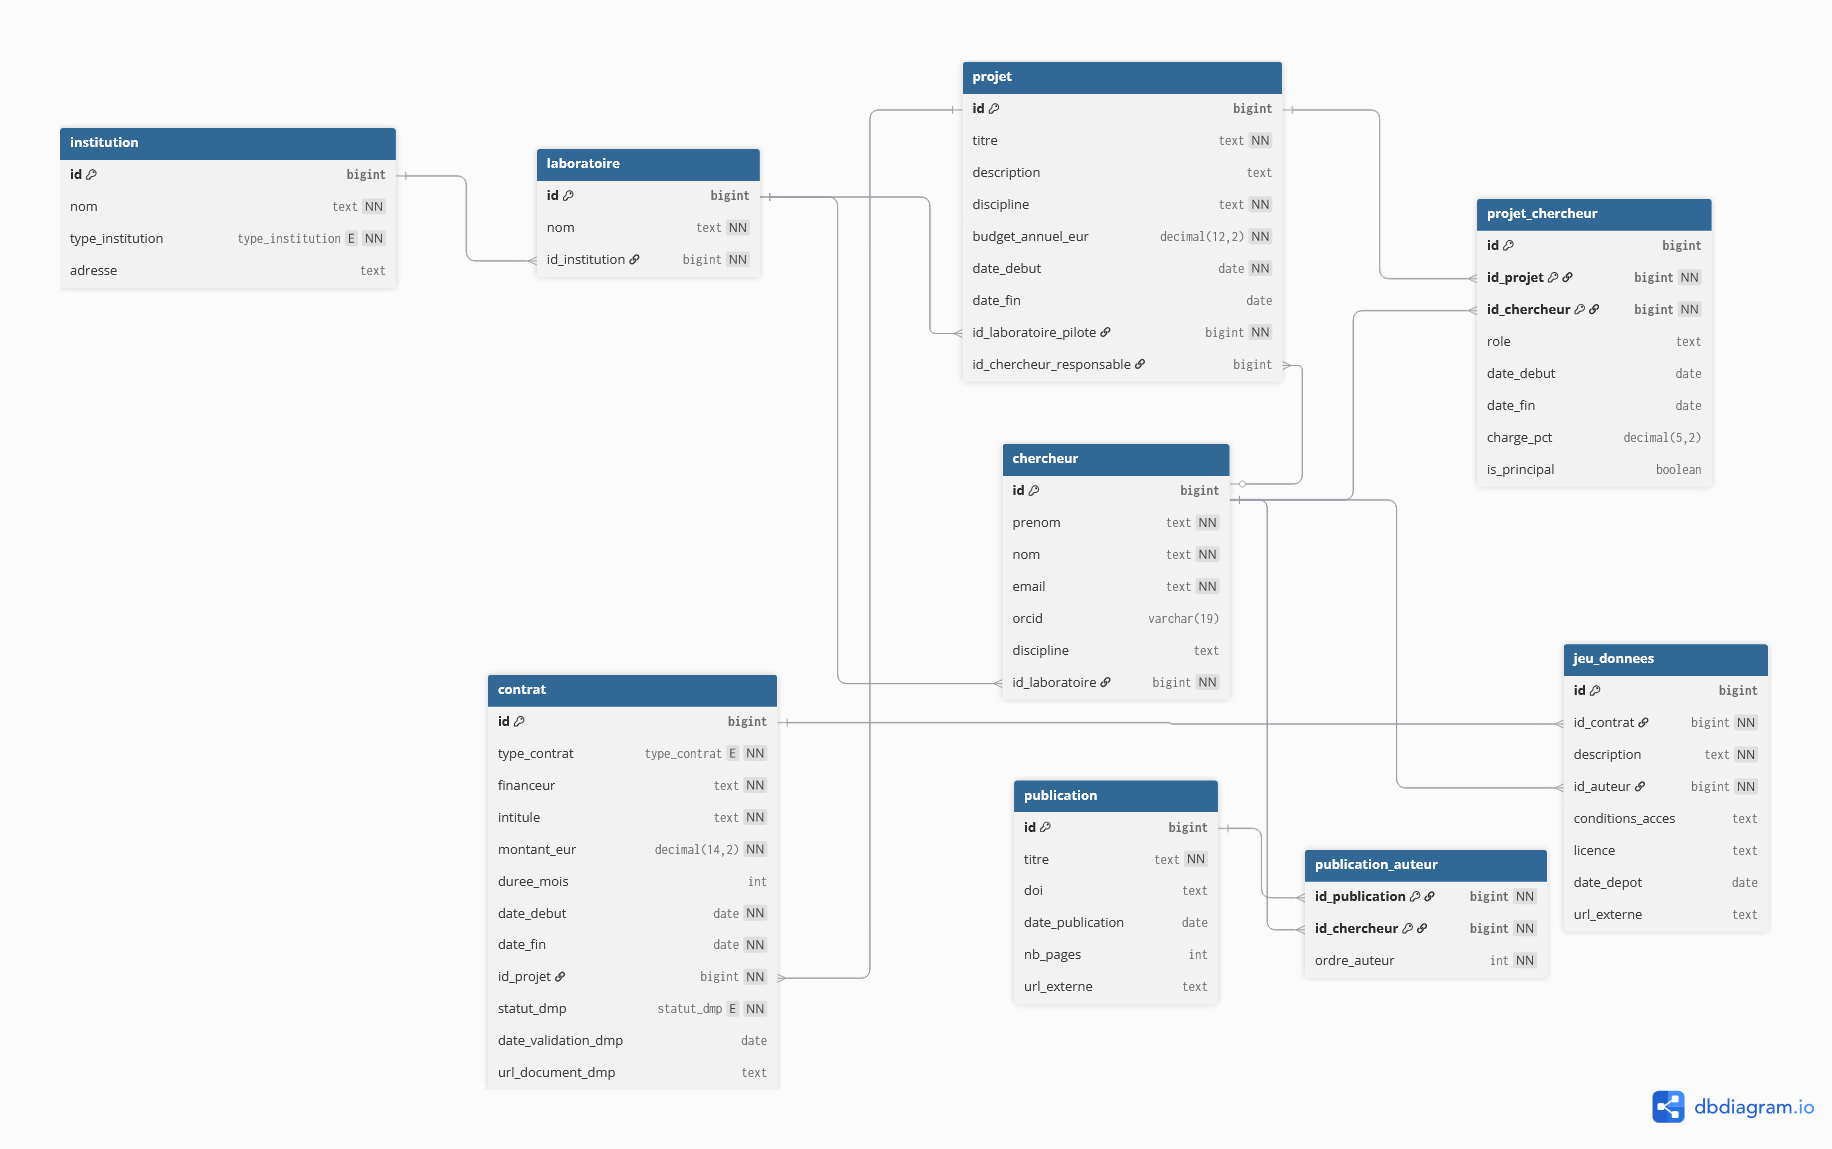
\includegraphics[width=\textwidth]{../infos/schema_img.png}
    \caption{Schéma relationnel de la base de données. Effectué sur \href{https://dbdiagram.io/}{DBDiagram.io}. En utilisant le langage DBML.}
    \label{fig:schema}
\end{figure}

\subsubsection{Contraintes CHECK}
\begin{itemize}
    \item Vérification que budget\_annuel\_eur $\geq$ 0
    \item Vérification que montant\_eur $\geq$ 0
    \item Vérification que date\_fin $\geq$ date\_debut
    \item Validation du statut DMP et de ses champs associés
\end{itemize}

\newpage

% Partie 2
\section{Partie 2 - Peuplement de la Base de Données}

\subsection{Méthodologie}

\subsubsection{Outils utilisés}
\begin{itemize}
    \item Python 3.x
    \item Bibliothèque Faker
    \item PostgreSQL
\end{itemize}

\subsubsection{Démarche générale}
Pour mener à bien ce générateur de données, nous avons tout d'abord analysés les types de données nécessaires pour chaque table, ainsi que les contraintes d'intégrité référentielle.

Dans notre cas, nous avions besoin de générer des emails, des dates cohérentes, des montants financiers, des identifiants uniques, de faux noms et prénoms, des titres de projets et publications, etc.

Pour ce faire, la simple utilisation de la Bibliothèque Faker nous a permis de générer la majorité des données de manière réaliste. Le reste des données spécifiques (comme les types de contrats, le statut DMP, etc.) ont été gérées par des listes prédéfinies.

Ensuite, nous avons structuré le script Python pour générer les données dans un ordre respectant les dépendances entre les tables (par exemple, générer les institutions avant les laboratoires, etc.).

L'analyse des contraintes d'intégrité est la partie la plus délicate, car il faut s'assurer que les clés étrangères pointent vers des enregistrements existants, et que les données respectent les contraintes de dates et autres règles métier. Le tout dans un code maintenable, modulaire et clair, pour faciliter les modifications futures.

\subsection{Architecture du script Python}

\subsubsection{Structure du code}
Le script Python est organisé en plusieurs fonctions modulaires qui génèrent les données de manière séquentielle en respectant les dépendances :

\begin{itemize}
    \item \textbf{Fonctions utilitaires} :
    \begin{itemize}
        \item \texttt{\_quote\_sql()} : Échappement sécurisé des valeurs SQL;
        \item \texttt{gen\_orcid()} : Génération d'identifiants ORCID au format standard;
        \item \texttt{random\_date\_between()} : Génération de dates cohérentes dans un intervalle.
    \end{itemize}
    
    \item \textbf{Fonction d'en-tête} :
    \begin{itemize}
        \item \texttt{write\_header()} : Inclusion du schéma et initialisation de la transaction.
    \end{itemize}
    
    \item \textbf{Fonctions de génération par table} (dans l'ordre des dépendances) :
    \begin{itemize}
        \item \texttt{generate\_institutions()} : Création des institutions avec types variés;
        \item \texttt{generate\_laboratoires()} : Rattachement aux institutions avec noms uniques;
        \item \texttt{generate\_chercheurs()} : Génération avec emails et ORCID uniques;
        \item \texttt{generate\_projets()} : Attribution de responsables et dates cohérentes;
        \item \texttt{generate\_contrats()} : Gestion des statuts DMP et retour des contrats validés;
        \item \texttt{generate\_jeux\_donnees()} : Respect des contraintes DMP (dépôt uniquement si validé);
        \item \texttt{generate\_publications()} : Création avec DOI uniques et auteurs multiples;
        \item \texttt{generate\_projet\_chercheur()} : Table associative N-N avec rôles et charges.
    \end{itemize}
    
    \item \textbf{Fonction principale} :
    \begin{itemize}
        \item \texttt{main()} : Orchestration de l'ensemble du processus de génération.
    \end{itemize}
\end{itemize}

Le script utilise un système de retour des identifiants générés pour garantir la cohérence référentielle entre les tables. Chaque fonction retourne la liste des IDs créés, qui sont ensuite utilisés comme clés étrangères par les fonctions suivantes.

\subsubsection{Gestion de l'intégrité référentielle}
Nous avons mis en place plusieurs mécanismes pour garantir l'intégrité référentielle et le respect des différentes contraintes :

\begin{itemize}
    \item \textbf{Propagation des IDs} : Chaque fonction de génération retourne la liste des identifiants créés, qui sont passés en paramètre aux fonctions suivantes
    
    \item \textbf{Gestion des contraintes d'unicité} :
    \begin{itemize}
        \item Utilisation de sets Python (\texttt{emails\_used}, \texttt{orcids\_used}, \texttt{dois\_used}) pour éviter les doublons;
        \item Système de tentatives multiples (jusqu'à 100 tentatives pour trouver une valeur unique sinon mise à \texttt{null}) pour générer des valeurs uniques;
        \item Mécanisme de fallback avec suffixes numériques en cas d'échec.
    \end{itemize}
    
    \item \textbf{Respect des contraintes temporelles} :
    \begin{itemize}
        \item Vérification que \texttt{date\_fin} $\geq$ \texttt{date\_debut} pour les projets et contrats;
        \item Génération de dates de validation DMP postérieures au début du contrat;
        \item Cohérence des dates de participation chercheur-projet.
    \end{itemize}
    
    \item \textbf{Respect des règles métier} :
    \begin{itemize}
        \item Dépôt de jeux de données uniquement pour les contrats avec DMP validé;
        \item Attribution de chercheurs responsables existants aux projets;
        \item Génération de noms de laboratoires uniques par institution.
    \end{itemize}
    
    \item \textbf{Mise à jour des séquences} : Réinitialisation automatique des séquences PostgreSQL après chaque table avec \texttt{setval()} pour permettre des insertions manuelles ultérieures.
\end{itemize}

\subsection{Génération des données par table}

\subsubsection{Institutions}
\begin{itemize}
    \item \textbf{Nombre généré} : Paramétrable, par défaut $\max(3, \lfloor rows/10 \rfloor)$;
    \item Génération via \texttt{fake.company()} avec types variés (université, organisme de recherche, partenaire privé);
    \item \textbf{Exemple} : "Martin Technologies", type "partenaire\_prive", adresse "12 rue de la Paix, 75002 Paris".
\end{itemize}

\subsubsection{Laboratoires}
\begin{itemize}
    \item \textbf{Nombre généré} : $\max(5, \lfloor rows/8 \rfloor)$;
    \item Rattachement d'une institution aléatoire avec garantie d'unicité des noms par institution;
    \item \textbf{Exemple} : "Deliver innovative Lab", rattaché à l'institution 2.
\end{itemize}

\subsubsection{Chercheurs}
\begin{itemize}
    \item \textbf{Nombre généré} : $\max(20, rows)$ (paramètre principal);
    \item \textbf{Attributs générés} :
    \begin{itemize}
        \item Email unique construit à partir du prénom et nom;
        \item ORCID unique généré pour 50\% des chercheurs (format XXXX-XXXX-XXXX-XXXX);
        \item Discipline parmi 5 domaines (Physique, Biologie, Informatique, Chimie, Mathématiques).
    \end{itemize}
    \item \textbf{Cohérence} : Rattachement aléatoire mais cohérent à un laboratoire existant;
    \item \textbf{Exemple} : Marie Dubois, marie.dubois@example.com, ORCID 1234-5678-9012-3456, discipline Informatique.
\end{itemize}

\subsubsection{Projets}
\begin{itemize}
    \item \textbf{Nombre généré} : $\max(10, \lfloor rows/5 \rfloor)$;
    \item Sélection aléatoire d'un chercheur existant pour le chercheur responsable (peut être NULL);
    \item Date de début entre -5 ans et aujourd'hui, date de fin entre date\_debut et +3 ans;
    \item Montants réalistes du budget (entre 10\,000€ et 500\,000€);
    \item \textbf{Exemple} : "Optimize cross-platform networks", budget 125\,000€, du 2020-03-15 au 2023-12-31.
\end{itemize}

\subsubsection{Contrats}
\begin{itemize}
    \item \textbf{Nombre généré} : $\max(10, \lfloor rows/4 \rfloor)$;
    \item Distribution des types réaliste entre ANR, H2020, Région, Europe, Autre;
    \item Montants Entre 10\,000€ et 2\,000\,000€;
    \item \textbf{Gestion DMP} :
    \begin{itemize}
        \item Statuts pondérés : 50\% brouillon, 30\% soumis, 20\% validé;
        \item Date de validation et URL uniquement pour les contrats validés;
        \item Retour séparé des contrats validés pour les jeux de données.
    \end{itemize}
\end{itemize}

\subsubsection{Publications}
\begin{itemize}
    \item \textbf{Nombre généré} : $\max(10, \lfloor rows/5 \rfloor)$;
    \item Génération unique de DOI pour 40\% des publications (format 10.XXXX/XXXXXX);
    \item Entre 1 et 5 auteurs par publication avec ordre de signature;
    \item Métadonnées : Date de publication, nombre de pages, URL externe (HAL);
    \item \textbf{Exemple} : "Impact of climate on biodiversity", DOI 10.1234/abc123, 3 auteurs, 15 pages.
\end{itemize}

\subsubsection{Jeux de données}
\begin{itemize}
    \item \textbf{Nombre généré} : $\max(5, \lfloor rows/6 \rfloor)$;
    \item Date de dépôt générée uniquement pour les contrats avec DMP validé (40\% des cas);
    \item Distribution des Licences entre CC-BY, CC0, ODbL ou NULL;
    \item Conditions d'accès entre Ouvert, restreint ou sur demande;
    \item \textbf{Exemple} : Dataset associé au contrat validé 15, licence CC-BY, déposé le 2024-05-12.
\end{itemize}

\subsection{Cohérence des données générées}

Les données générées respectent plusieurs niveaux de cohérence :

\begin{enumerate}
    \item \textbf{Cohérence temporelle} : Toutes les dates respectent les contraintes CHECK (date\_fin $\geq$ date\_debut)
    
    \item \textbf{Cohérence référentielle} : Toutes les clés étrangères pointent vers des enregistrements existants grâce au système de propagation des IDs
    
    \item \textbf{Cohérence métier} :
    \begin{itemize}
        \item Les jeux de données avec date\_depot sont liés à des contrats DMP validés
        \item Les chercheurs responsables de projets appartiennent à des laboratoires existants
        \item Les auteurs de publications sont des chercheurs référencés
        \item L'ordre des auteurs est unique par publication
    \end{itemize}
    
    \item \textbf{Unicité garantie} : Emails, ORCID, DOI sont uniques grâce aux mécanismes de détection de doublons
    
    \item \textbf{Réalisme des données} : Utilisation de Faker avec locale française pour des noms, adresses et domaines cohérents
\end{enumerate}

\subsubsection{Statistiques des données générées}
Tableau récapitulatif du nombre d'enregistrements par table pour un paramètre \texttt{nb\_rows} fixé à 50\,000.

\begin{table}[H]
\centering
\begin{tabular}{@{}lc@{}}
\toprule
\textbf{Table} & \textbf{Nombre d'enregistrements} \\ \midrule
Institution & 5\,000 \\
Laboratoire & 6\,250 \\
Chercheur & 50\,000 \\
Projet & 10\,000 \\
Contrat & 12\,460 \\
Publication & 10\,000 \\
Publication\_Auteur & 29\,818 \\
Jeu\_Donnees & 6\,150 \\ \bottomrule
\end{tabular}
\caption{Statistiques des données générées pour 50\,000 chercheurs.}
\label{tab:stats}
\end{table}

\subsection{Exemples de code}

\subsubsection{Génération des projets}
\begin{lstlisting}[style=pythonstyle, caption=Exemple de génération des projets]
def generate_projets(f, fake: Faker, laboratoires: List[int], chercheurs: List[int], count: int) -> List[int]:
    """Genere les projets et retourne la liste des IDs."""
    projets = []
    
    for pid in range(1, count + 1):
        titre = fake.catch_phrase()
        description = fake.paragraph(nb_sentences=3)
        discipline = random.choice(["Physique", "Biologie", "Informatique", "Chimie", "Mathematiques"])
        budget = round(random.uniform(10000, 500000), 2)
        d_debut = fake.date_between(start_date='-5y', end_date='today')
        d_fin = None if random.random() < 0.2 else fake.date_between(start_date=d_debut, end_date='+3y')
        id_labo = random.choice(laboratoires)
        id_resp = random.choice(chercheurs) if chercheurs else None
        projets.append(pid)
        f.write(f"INSERT INTO univ_recherche.projet (id, titre, description, discipline, budget_annuel_eur, date_debut, date_fin, id_laboratoire_pilote, id_chercheur_responsable) VALUES ({pid}, {_quote_sql(titre)}, {_quote_sql(description)}, {_quote_sql(discipline)}, {budget}, {_quote_sql(d_debut)}, {_quote_sql(d_fin)}, {id_labo}, {_quote_sql(id_resp)});\n")
    
    f.write("SELECT setval(pg_get_serial_sequence('univ_recherche.projet','id'), COALESCE((SELECT MAX(id) FROM univ_recherche.projet),0));\n")
    return projets
\end{lstlisting}

\subsubsection{Génération des chercheurs}
\begin{lstlisting}[style=pythonstyle, caption=Exemple de génération des chercheurs]
def generate_chercheurs(f, fake: Faker, laboratoires: List[int], count: int) -> List[int]:
    """Genere les chercheurs et retourne la liste des IDs."""
    chercheurs = []
    emails_used = set()
    orcids_used = set()
    
    for cid in range(1, count + 1):
        prenom = fake.first_name()
        nom = fake.last_name()
        
        # Generer un email unique
        attempts = 0
        while attempts < 100:
            if attempts == 0:
                email = (prenom + "." + nom + "@" + fake.domain_name()).lower()
            else:
                email = (prenom + "." + nom + str(attempts) + "@" + fake.domain_name()).lower()
            if email not in emails_used:
                emails_used.add(email)
                break
            attempts += 1
        else:
            # Fallback: email avec ID unique
            email = f"chercheur{cid}@" + fake.domain_name()
            emails_used.add(email)
        
        # Generer un ORCID unique ou NULL
        orcid = None
        if random.random() < 0.5:
            attempts = 0
            while attempts < 100:
                orcid_candidate = gen_orcid(fake)
                if orcid_candidate not in orcids_used:
                    orcids_used.add(orcid_candidate)
                    orcid = orcid_candidate
                    break
                attempts += 1
        
        discipline = random.choice(["Physique", "Biologie", "Informatique", "Chimie", "Mathematiques"])
        id_labo = random.choice(laboratoires)
        chercheurs.append(cid)
        f.write(f"INSERT INTO univ_recherche.chercheur (id, prenom, nom, email, orcid, discipline, id_laboratoire) VALUES ({cid}, {_quote_sql(prenom)}, {_quote_sql(nom)}, {_quote_sql(email)}, {_quote_sql(orcid)}, {_quote_sql(discipline)}, {id_labo});\n")
    
    f.write("SELECT setval(pg_get_serial_sequence('univ_recherche.chercheur','id'), COALESCE((SELECT MAX(id) FROM univ_recherche.chercheur),0));\n")
    return chercheurs
\end{lstlisting}

\newpage

% Partie 3
\section{Partie 3 - Gestion des Utilisateurs et Création de Vues}

\subsection{Stratégie de sécurité}

\subsubsection{Objectifs}
Pour pouvoir mettre en oeuvre une base de données réaliste, elle doit être sécurisée. Nous avons alors, en suivant rigoureusement les besoins de l'énoncés, mis en place une stratégie de sécurité basée sur la gestion des rôles et des privilèges.

\subsubsection{Architecture des rôles}
Nous avons défini trois rôles principaux pour gérer les accès à la base de données :
\begin{itemize}
    \item \textbf{Chercheur} : Accès restreint aux données liées à ses propres projets et publications.
    \item \textbf{Data Manager} : Accès élargi aux métadonnées des jeux de données et DMP, mais sans droits de suppression.
    \item \textbf{Administrateur} : Accès complet à toutes les données et fonctionnalités de la base.
\end{itemize}

\subsection{Définition des rôles}

\subsubsection{Rôle Chercheur}
\begin{itemize}
    \item Description : Accès restreint aux données du chercheur
    \item Privilèges : SELECT, INSERT, UPDATE sur ses propres données
    \item Restrictions : Pas d'accès aux données des autres chercheurs
\end{itemize}

\subsubsection{Rôle Data Manager}
\begin{itemize}
    \item Description : Accès élargi aux métadonnées
    \item Privilèges : SELECT sur toutes les tables, INSERT/UPDATE sur jeux de données et DMP
    \item Restrictions : Pas de suppression de données
\end{itemize}

\subsubsection{Rôle Administrateur}
\begin{itemize}
    \item Description : Accès complet
    \item Privilèges : ALL PRIVILEGES
    \item Responsabilités : Gestion complète de la base
\end{itemize}

\subsection{Vues créées}

\subsubsection{Vue 1 : Mes\_Projets}
\begin{itemize}
    \item Objectif : Permettre à un chercheur de voir ses projets
    \item Utilisateurs cibles : Chercheurs
    \item Contenu : Projets auxquels le chercheur participe
\end{itemize}

\begin{lstlisting}[style=sqlstyle, caption=Vue Mes\_Projets]
CREATE OR REPLACE VIEW v_mes_projets AS
SELECT 
    p.id AS projet_id,
    p.titre,
    p.discipline,
    p.date_debut,
    p.date_fin,
    p.budget_annuel_eur,
    l.nom AS laboratoire,
    CONCAT(resp.prenom, ' ', resp.nom) AS responsable,
    pc.role AS mon_role,
    pc.charge_pct
FROM projet p
JOIN laboratoire l ON p.id_laboratoire_pilote = l.id
JOIN projet_chercheur pc ON p.id = pc.id_projet
LEFT JOIN chercheur resp ON p.id_chercheur_responsable = resp.id
WHERE pc.id_chercheur = (SELECT id FROM chercheur WHERE email = current_user);
\end{lstlisting}

\subsubsection{Vue 2 : Metadata\_Jeux\_Donnees}
\begin{itemize}
    \item Objectif : Vue complète des métadonnées des jeux de données
    \item Utilisateurs cibles : Data Managers
    \item Contenu : Toutes les informations sur les jeux de données
\end{itemize}

\subsubsection{Vue 3 : Publications\_Par\_Laboratoire}
\begin{itemize}
    \item Objectif : Statistiques des publications par laboratoire
    \item Utilisateurs cibles : Administrateurs, Data Managers
\end{itemize}

\subsubsection{Vue 4 : Contrats\_Actifs}
\begin{itemize}
    \item Objectif : Liste des contrats en cours
    \item Utilisateurs cibles : Tous les rôles
\end{itemize}

\subsubsection{Vue 5 : Projets\_Budget\_Global}
\begin{itemize}
    \item Objectif : Vue agrégée des budgets par projet
    \item Utilisateurs cibles : Administrateurs
\end{itemize}

Voir Annexe pour le code SQL complet des vues.

\subsection{Attribution des privilèges}

\subsubsection{Privilèges par rôle}
Tableau récapitulatif des privilèges accordés à chaque rôle.

\begin{table}[H]
\centering
\begin{tabular}{@{}lccc@{}}
\toprule
\textbf{Vue/Table} & \textbf{Chercheur} & \textbf{Data Manager} & \textbf{Admin} \\ \midrule
mes\_projets & SELECT & SELECT & ALL \\
metadata\_jeux\_donnees & - & SELECT, INSERT & ALL \\
publications\_par\_labo & - & SELECT & ALL \\
contrats\_actifs & SELECT & SELECT & ALL \\
projets\_budget\_global & - & - & ALL \\ \bottomrule
\end{tabular}
\caption{Attribution des privilèges par rôle}
\label{tab:privileges}
\end{table}

\subsubsection{Exemples de scripts SQL}
\begin{lstlisting}[style=sqlstyle, caption=Création des rôles et attribution des privilèges]
-- Role Chercheur
CREATE ROLE role_chercheur;

-- Role Data Manager
CREATE ROLE role_data_manager;

-- Role Administrateur
CREATE ROLE role_administrateur;

-- Creation des vues, etc. (voir sections precedentes)

-- Privileges pour ADMINISTRATEUR
GRANT ALL PRIVILEGES ON ALL TABLES IN SCHEMA univ_recherche TO role_administrateur;
GRANT ALL PRIVILEGES ON ALL SEQUENCES IN SCHEMA univ_recherche TO role_administrateur;
GRANT EXECUTE ON ALL FUNCTIONS IN SCHEMA univ_recherche TO role_administrateur;

-- Privileges pour DATA_MANAGER
GRANT SELECT ON ALL TABLES IN SCHEMA univ_recherche TO role_data_manager;
GRANT INSERT, UPDATE, DELETE ON contrat, jeu_donnees TO role_data_manager;
GRANT SELECT ON v_metadonnees_contrats, v_synthese_donnees_projet, v_tableau_bord_projets TO role_data_manager;
GRANT SELECT ON v_publications_chercheur TO role_data_manager;

-- Privileges pour CHERCHEUR
GRANT SELECT ON projet, chercheur, laboratoire, institution, publication TO role_chercheur;
GRANT SELECT ON v_mes_projets, v_mes_donnees, v_publications_chercheur TO role_chercheur;
GRANT INSERT ON publication, publication_auteur, jeu_donnees TO role_chercheur;
GRANT UPDATE ON jeu_donnees TO role_chercheur;

\end{lstlisting}

\newpage

% Partie 4
\section{Partie 4 - Requêtes et Optimisation}

\subsection{Méthodologie d'optimisation}

\subsubsection{Démarche}
\begin{enumerate}
    \item Écriture de plusieurs versions de chaque requête
    \item Analyse des plans d'exécution
    \item Comparaison des performances et des méthodes utilisées par le SGBD
    \item Création d'index ciblés
    \item Validation des améliorations
\end{enumerate}

\subsection{Requête R1 - Jeux de données par projet}

\subsubsection{Énoncé}
Nombre total de jeux de données déposés par projet et par année civile, ainsi que la moyenne du délai de dépôt (en jours) pour les projets ayant impliqué > 5 chercheurs depuis 2018.

\subsubsection{Version 1}
\begin{lstlisting}[style=sqlstyle, caption=R1 - Version 1]
-- Code SQL Version 1
\end{lstlisting}

\subsubsection{Version 2}
\begin{lstlisting}[style=sqlstyle, caption=R1 - Version 2]
-- Code SQL Version 2
\end{lstlisting}

\subsubsection{Analyse des performances}
\begin{itemize}
    \item Temps d'exécution Version 1 : XX ms
    \item Temps d'exécution Version 2 : XX ms
    \item Opérations coûteuses identifiées
\end{itemize}

\subsubsection{Plans d'exécution}
Captures d'écran et analyse des plans EXPLAIN ANALYZE.

\subsubsection{Optimisation choisie}
Justification du choix de la version retenue et description des index créés.

\begin{lstlisting}[style=sqlstyle, caption=Index pour R1]
-- Code SQL des index
\end{lstlisting}

\subsection{Requête R2 - Projets sans chercheurs peu productifs}

\subsubsection{Énoncé}
Pour le laboratoire LISA en 2024, donner la liste des projets et le nom du responsable qui n'ont aucun chercheur dont le nombre de publications en 2024 est strictement inférieur à la moyenne.

\subsubsection{Version 1}
\begin{lstlisting}[style=sqlstyle, caption=R2 - Version 1]
-- Code SQL Version 1
\end{lstlisting}

\subsubsection{Version 2}
\begin{lstlisting}[style=sqlstyle, caption=R2 - Version 2]
-- Code SQL Version 2
\end{lstlisting}

\subsubsection{Analyse des performances}
Comparaison des deux versions.

\subsubsection{Plans d'exécution}
Analyse détaillée.

\subsubsection{Optimisation choisie}
Justification et index.

\subsection{Requête R3 - Laboratoires conformes}

\subsubsection{Énoncé}
Laboratoires n'ayant eu aucun jeu de données non conforme en 2024 (sans licence ou sans date\_depot).

\subsubsection{Version 1}
\begin{lstlisting}[style=sqlstyle, caption=R3 - Version 1]
-- Code SQL Version 1
\end{lstlisting}

\subsubsection{Version 2}
\begin{lstlisting}[style=sqlstyle, caption=R3 - Version 2]
-- Code SQL Version 2
\end{lstlisting}

\subsubsection{Analyse des performances}
Comparaison détaillée.

\subsubsection{Plans d'exécution}
Captures et analyse.

\subsubsection{Optimisation choisie}
Justification et index.

\subsection{Synthèse des optimisations}

\subsubsection{Index créés}
Liste récapitulative de tous les index créés avec leur justification.

\begin{table}[H]
\centering
\begin{tabular}{@{}lll@{}}
\toprule
\textbf{Table} & \textbf{Colonnes} & \textbf{Justification} \\ \midrule
jeu\_donnees & (date\_depot) & Filtrage par année \\
chercheur & (id\_projet) & Jointures fréquentes \\
publication\_auteur & (id\_chercheur, date) & Comptage publications \\ \bottomrule
\end{tabular}
\caption{Index créés pour l'optimisation}
\label{tab:index}
\end{table}

\subsubsection{Gains de performance}
Tableau comparatif des temps d'exécution avant et après optimisation.

\newpage

% Partie 5
\section{Partie 5 - Triggers et Procédures Stockées}

\subsection{Triggers}

\subsubsection{Trigger 1 : Limite de participants à un projet}

\paragraph{Objectif}
Vérifier lors de l'insertion d'une participation qu'on ne dépasse pas la capacité maximale du projet.

\paragraph{Implémentation}
\begin{lstlisting}[style=sqlstyle, caption=Trigger limite participants]
-- Code SQL du trigger
\end{lstlisting}

\paragraph{Tests}
Description des tests effectués et résultats.

\subsubsection{Trigger 2 : Vérification DMP d'un jeu de données}

\paragraph{Objectif}
Empêcher le passage d'un jeu de données en statut "déposé" si le DMP du contrat n'est pas validé.

\paragraph{Implémentation}
\begin{lstlisting}[style=sqlstyle, caption=Trigger vérification DMP]
-- Code SQL du trigger
\end{lstlisting}

\paragraph{Tests}
Scénarios de test et résultats.

\subsection{Procédures stockées et fonctions}

\subsubsection{Fonction 1 : Nombre de publications d'un projet}

\paragraph{Objectif}
Calculer le nombre de publications pour un projet donné et une année donnée.

\paragraph{Signature}
\begin{lstlisting}[style=sqlstyle, caption=Signature de la fonction]
CREATE FUNCTION nb_publications_projet(
    p_id_projet BIGINT,
    p_annee INTEGER
) RETURNS INTEGER
\end{lstlisting}

\paragraph{Implémentation}
\begin{lstlisting}[style=sqlstyle, caption=Fonction nb\_publications\_projet]
-- Code SQL complet
\end{lstlisting}

\paragraph{Tests}
\begin{lstlisting}[style=sqlstyle, caption=Tests de la fonction]
-- Scripts de test
\end{lstlisting}

\subsubsection{Procédure 2 : Préparation du bilan d'un projet}

\paragraph{Objectif}
Mettre à jour une table de bilan avec le nombre de publications et jeux de données par projet pour une année donnée.

\paragraph{Table de bilan}
\begin{lstlisting}[style=sqlstyle, caption=Table bilan\_projet]
-- Structure de la table
\end{lstlisting}

\paragraph{Implémentation}
\begin{lstlisting}[style=sqlstyle, caption=Procédure preparation\_bilan]
-- Code SQL complet
\end{lstlisting}

\paragraph{Tests}
Scripts de test et résultats.

\subsubsection{Fonction 3 : Fiche projet}

\paragraph{Objectif}
Renvoyer la liste des publications et jeux de données associés à un projet avec leurs principales informations.

\paragraph{Type de retour}
Description de la structure retournée (TABLE, SETOF, JSON, etc.).

\paragraph{Implémentation}
\begin{lstlisting}[style=sqlstyle, caption=Fonction fiche\_projet]
-- Code SQL complet
\end{lstlisting}

\paragraph{Tests}
Exemples d'utilisation et résultats.

\subsubsection{Procédure 4 : Archivage des contrats échus}

\paragraph{Objectif}
Déplacer les contrats dont la date de fin est antérieure à une date seuil dans une table d'archives.

\paragraph{Table d'archives}
\begin{lstlisting}[style=sqlstyle, caption=Table contrat\_archive]
-- Structure de la table
\end{lstlisting}

\paragraph{Implémentation}
\begin{lstlisting}[style=sqlstyle, caption=Procédure archivage\_contrats]
-- Code SQL complet
\end{lstlisting}

\paragraph{Tests}
Scripts de test avec différentes dates seuil.

\subsection{Documentation du code}

\subsubsection{Conventions de nommage}
Description des conventions adoptées pour les variables, paramètres, etc.

\subsubsection{Commentaires}
Exemples de commentaires dans le code PL/pgSQL.

\newpage

% Conclusion
\section{Conclusion}

\subsection{Synthèse du travail réalisé}
Récapitulatif des différentes parties et des résultats obtenus.

\subsection{Apports pédagogiques}

\subsubsection{Compétences techniques acquises}
\begin{itemize}
    \item Conception de schéma relationnel complexe
    \item Maîtrise de PostgreSQL et PL/pgSQL
    \item Techniques d'optimisation de requêtes
    \item Gestion de la sécurité et des accès
\end{itemize}

\subsubsection{Utilisation de l'IA générative}
Retour critique sur l'utilisation des outils d'IA dans le processus de développement.

\subsection{Difficultés rencontrées}
Liste des principaux défis et solutions apportées.

\subsection{Perspectives d'amélioration}
Pistes d'amélioration pour la base de données et le processus de développement.

\newpage

% Annexes
\appendix

\section{Scripts SQL}

\subsection{Script de création du schéma}
Référence au fichier \texttt{schema\_univ\_recherche.sql}.

\subsection{Script d'insertion des données}
Référence au fichier \texttt{inserts\_postgres.sql}.

\subsection{Script de gestion des utilisateurs}
Référence au fichier \texttt{schema\_avance.sql} Partie 3.

\subsection{Scripts des requêtes optimisées}
Référence au fichier \texttt{schema\_avance.sql} Partie 4.

\subsection{Scripts des triggers et procédures}
Référence au fichier \texttt{schema\_avance.sql} Partie 5.

\section{Code Python}

\subsection{Script de génération de données}
\label{sec:code-python}
    Référence au fichier \texttt{generate\_data.py}.

\section{Captures d'écran}

\subsection{Plans d'exécution}
Captures d'écran des plans EXPLAIN ANALYZE pour les requêtes optimisées.

\subsection{Tests des procédures}
Captures d'écran des résultats des tests.

\section{Dictionnaire de données}
Référence au fichier \texttt{dictionnaire\_attributs.md}.

\end{document}
